% +--------------------------------------------------------------------+
% | Sample Chapter 4
% +--------------------------------------------------------------------+

\cleardoublepage

% +--------------------------------------------------------------------+
% | Replace "This is Chapter 4" below with the title of your chapter.
% | LaTeX will automatically number the chapters.
% +--------------------------------------------------------------------+

\chapter{Implementación}
\label{makereference4}
Nuestra aplicación es una aplicación móvil desarrollada en Android, Unity y Vuforia y con un servidor desarrollado en Java usando Spring.
En este capítulo comenzaremos describiendo todos los prototipos de implementación que hemos desarrollado, en los cuáles veremos los pros y contras de las
tecnologías que hemos probado y el porqué de nuestra elección de implementar la aplicación con estas tecnologías. 
Después describiremos cómo hemos implementado nuestra aplicación, desde la arquitectura que hemos seguido, 
las tecnologías usadas para la parte frontend y la parte backend junto a las dificultades 
que nos hemos encontrado mientras trabajábamos. Finalmente hablaremos de las herramientas de trabajo
utilizadas para facilitarnos el trabajo en equipo.
\begin{center}
    \begin{tabularx}{1\textwidth}{@{\extracolsep{\fill}} | X | l | l |} \hline
    \multicolumn{3}{|l|}{Enlaces de GitHub } \\ \hline
    Aplicación & Licencia & Enlace \\ \hline
    Escena de AR en Unity con Vuforia & Apache-2.0 & \url{https://github.com/DanielCalle/TFG-Vuforia} \\ \hline
    Aplicación de Android & Apache-2.0 & \url{https://github.com/DanielCalle/TFG-Android} \\ \hline
    Servidor de Spring & Apache-2.0 & \url{https://github.com/DanielCalle/TFG-Server} \\ \hline
    \end{tabularx}
\end{center}
\section{Pruebas de arquitectura}
\label{makereference4.1}
Estas pruebas sirven para conocer si las tecnologías seleccionadas
de la \autoref{makereference2.1.1} son viables dentro de nuestro proyecto.
Desarrollaremos prototipos con funcionalidades básicas y evaluaremos las partes
positivas y negativas de dichas tecnologías. Esto nos permitirá decidir cuales
son las mejores opciones para construir el software.

\subsection{ARCore} 
\label{makereference4.1.1} 
    Al comenzar la fase de desarrollo de proyectos, pensamos que una de las tecnologías que debíamos 
    investigar y probar debía ser ARCore. Esto se debía a que, la empresa detrás de esta 
    tecnología es Google y esto podría significar que tendríamos más material de consulta 
    y ejemplos en comparación con otras tecnologías de fabricantes con menos recursos.
    ARCore se encuentra disponible para Java, Unity, Unreal e iOS. Comenzamos realizando el 
    "Quickstart"\ para Android y posteriormente para Unity. 
    Tras realizar los proyectos propuestos por ARCore, realizamos algún proyecto propio 
    para comprobar si la herramienta se ajustaba a la idea que teníamos para nuestro futuro proyecto.
    Tras realizar ambos proyectos, concluimos que, aunque ARCore reúne las características 
    necesarias para en un futuro convertirse en una de las tecnologías más importantes en Realidad Aumentada, 
    no íbamos a seleccionarla para nuestro proyecto por las siguientes razones:
    \begin{itemize}
        \item Dispone de mucha documentación para comenzar a usar la herramienta, pero poca para realizar tareas más complejas.
        \item Resulta muy útil para realizar superposiciones de modelos 3D sobre superficies. Sin embargo, una de las funcionalidades más importantes que nuestra aplicación requería era la interacción con la realidad aumentada mediante el uso de botones, imágenes y la carga dinámica de elementos para posicionar en la pantalla de Realidad Aumentada e interaccionar con el usuario. En este sentido ARCore no está, por el momento, tan preparada como otras tecnologías.
    \end{itemize}
\subsection{Viro Media} 
\label{makereference4.1.2}

El objetivo del prototipo realizado con Viro Media es reconocer imágenes almacenadas en el dispositivo para mostrar texto y
objetos virtuales. Además de probar tecnologías de desarrollo móvil web como en este caso React Native
para plataformas iOS y Android. Comenzamos construyendo una interfaz sencilla con botones que nos redirigen a la escena de Realidad Aumentada (ver \autoref{fig:nativeBase_android} y \autoref{fig:nativeBase_ios}).
Para esta interfaz utilizamos NativeBase que es una librería que nos permite
realizar una aplicación con apariencias de tipo iOS o Android según el dispositivo.

\begin{figure}[htb]
    \centering
    \makebox[0pt][c]{%
    \begin{minipage}[b]{0.5\linewidth}
    \centering
      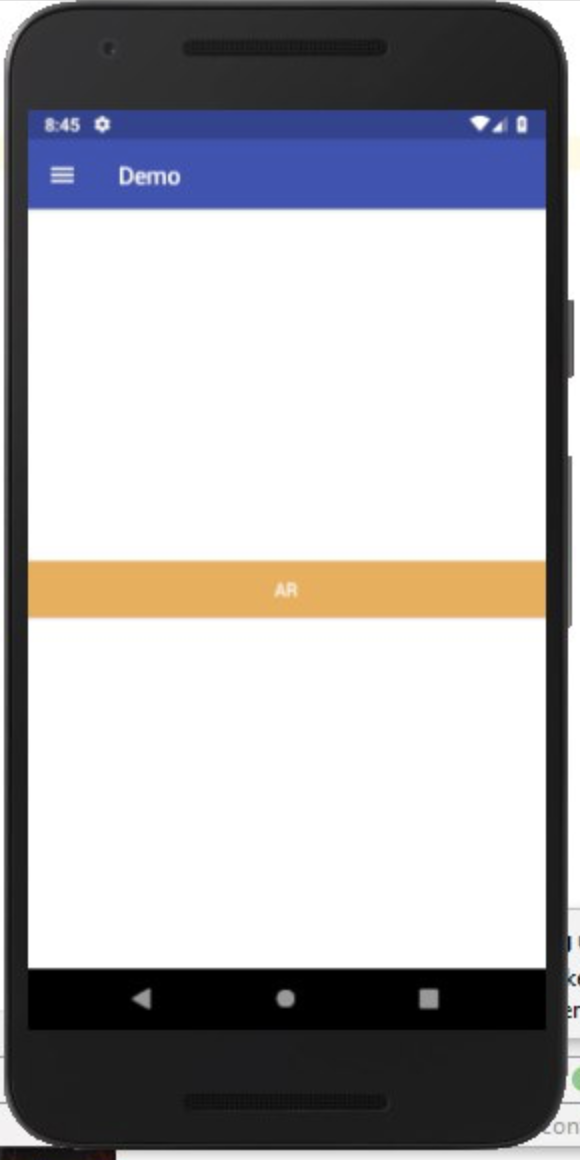
\includegraphics[scale=0.3]{figures/chapter-3/viromedia/android.png}
      \caption{Visualización con NativeBase en Android}
    \label{fig:nativeBase_android}
    \end{minipage}%
    \hspace{0.3cm}
    \begin{minipage}[b]{0.5\linewidth}
    \centering
     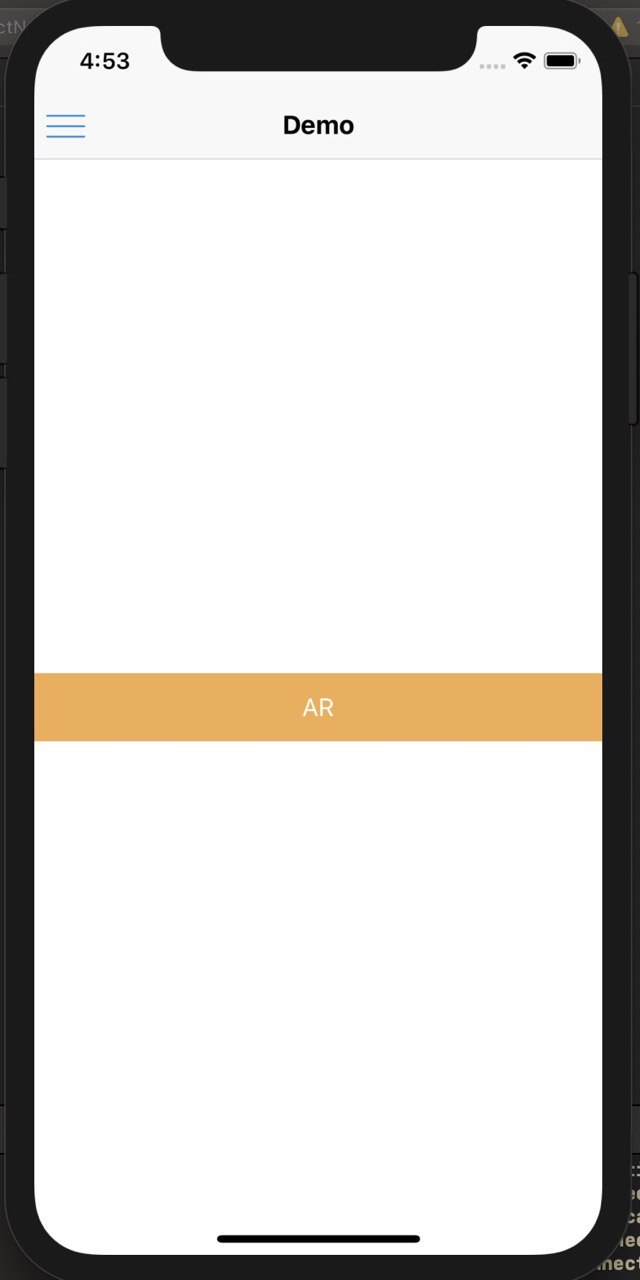
\includegraphics[scale=0.3]{figures/chapter-3/viromedia/ios.jpg}
      \caption{Visualización con NativeBase en iOS}
    \label{fig:nativeBase_ios}
    \end{minipage}%
    }%
\end{figure}

Para la escena de realidad aumentada mostramos texto y al detectar el póster de Pantera Negra,
reacciona mostrando una animación de dicho superhéroe saliendo del póster (ver \autoref{fig:visualizacionRANAtibe}).
 
\begin{figure}[H]
    \centering
    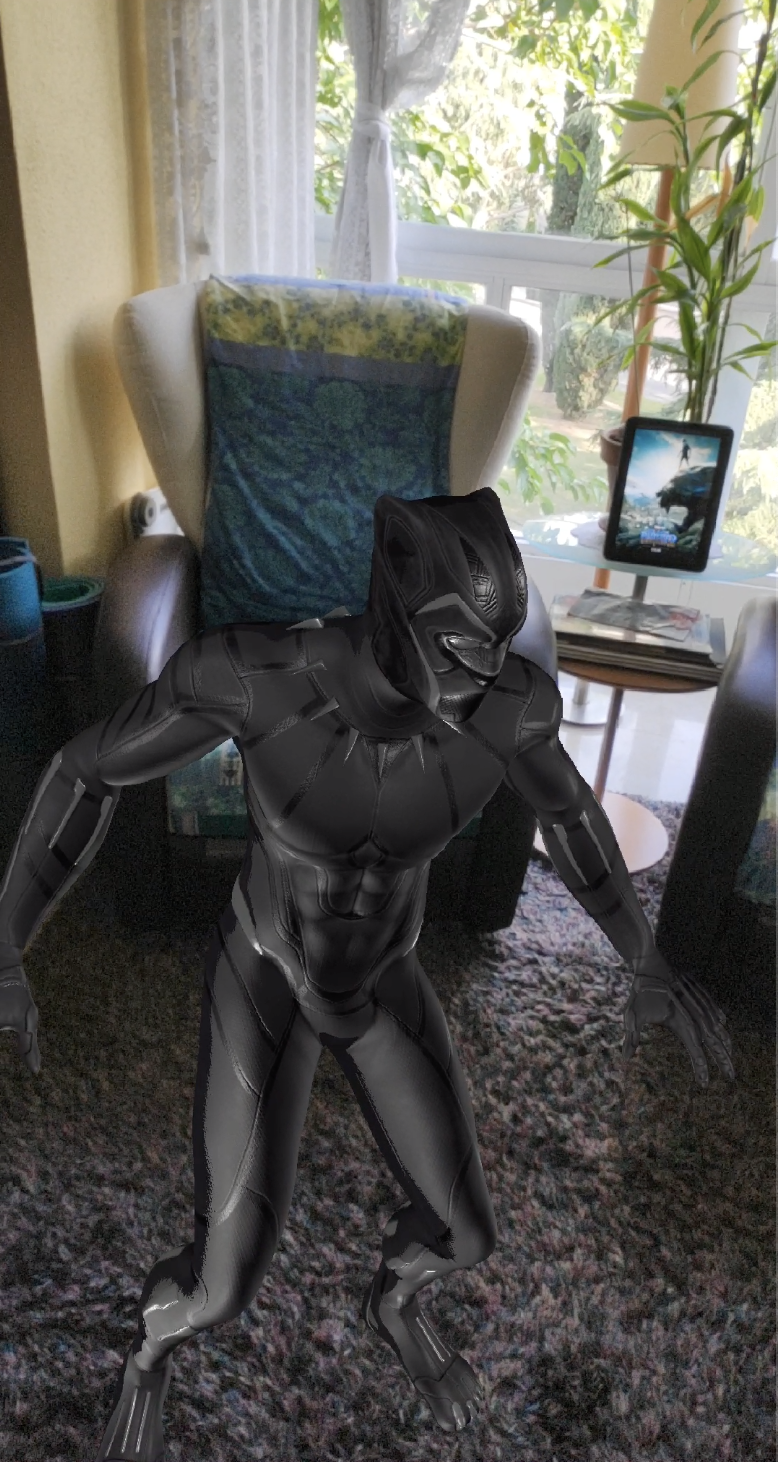
\includegraphics[height=4in]{figures/chapter-3/viromedia/blackpanther.png}
    \caption{Visualización de RA}
    \label{fig:visualizacionRANAtibe}
\end{figure}
\newpage
Una de las ventajas que apreciamos fue la facilidad del lenguaje, en este caso Javascript,
 utilizando la popular librería ReactJS y la buena documentación de Viro Media
 que hacían que el proceso de codificación fuera agradable.\\

Uno de los problemas que presentaba este prototipo era que las dependencias de Viro Media entraban en conflicto con las de NativeBase
imposibilitándonos la forma de encontrar versiones compatibles. Utilizamos las últimas que, a pesar de lanzar
 advertencias, funcionaba en el ejemplo realizado.
Otro problema fue la compilación de la aplicación, Viro Media tiene una aplicación para probar lo
 que desarrollamos conectándose a nuestro ordenador a través de la red. El problema es
 que algunos recursos, como los iconos que utilizaba NativeBase, no eran descargados, por lo que la
 mejor forma era probar la versión compilada de iOS y Android. La forma de compilar
 la aplicación era un proceso costoso para los ordenadores, lento y con multitud de problemas según
 se ampliaban las librerías que se utilizan.\\

La conclusión que obtuvimos de este prototipo fue que Viro Media y React Native son tecnologías muy prometedoras, pero debido a los
 problemas surgidos y a que todas sus versiones no eran estables vimos un claro riesgo para

\subsection{Vuforia + Android} 
\label{makereference4.1.3} 
 
En este prototipo utilizamos la librería nativa de Vuforia para Android para 
realizar las pruebas de tecnología de reconocimiento de imágenes tanto en  
local como usando la nube que nos ofrecía Vuforia, para la posterior renderización
de objetos y textos.

Las características tecnológicas de este prototipo son las siguientes:


\begin{enumerate}
    \item La librería de Vuforia para Android está diseñada a muy bajo nivel.
    \item Vuforia para dibujar en 3D usa la librería OpenGL (ver \autoref{fig:modelo3D}).
    \item OpenGL utiliza una serie de espacios donde se van colocando los elementos (ver \autoref{fig:esquemaOpenGl}): 
    \begin{enumerate}
        \item Local space: Es el espacio local de cada objeto.
        \item World space: Es el mundo donde se encuentran los objetos.
        \item View space: El mundo visto desde la perspectiva de la cámara.
        \item Clip space: Se integra con la pantalla del móvil y, definiendo los límites visibles, se establecen unas coordenadas de rango (-1,-1) - (1,1).
    \end{enumerate}
    
        Las transformaciones de estos espacios se realizan mediante matrices 4x4, 
        en las que la primera fila hace referencia a la coordenada $x$, la segunda a la coordenada $y$ y la 
        tercera a la coordenada $z$, mientras que la última columna hace referencia a los desplazamientos 
        de los objetos en esos 3 ejes.
            \begin{figure}[H]
                \centering
                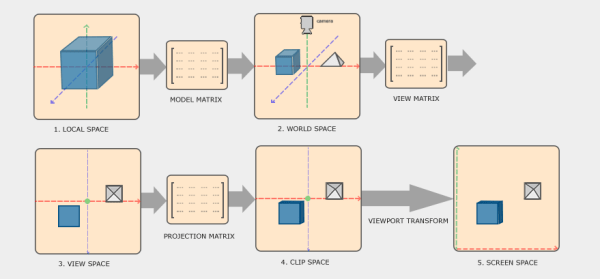
\includegraphics[width=5in]{figures/space-transformation.png}
                \caption{Esquema de los distintos espacios que usa OpenGL\cite{spaceopengl}}
                \label{fig:esquemaOpenGl}
            \end{figure}


            \begin{figure}[H]
                \centering
                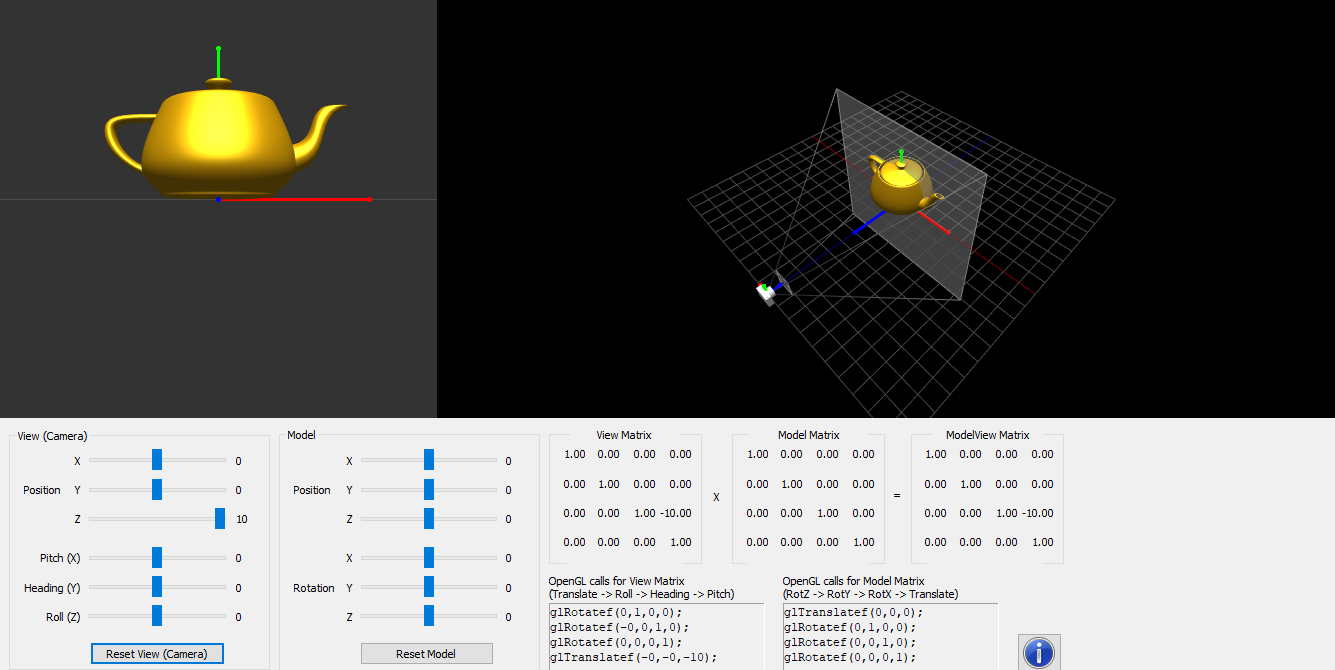
\includegraphics[width=5in]{figures/teapot.png}
                \caption{Captura de un ejemplo de un modelo en 3D}
                \label{fig:modelo3D}
            \end{figure}

    
    \item En OpenGL es necesario escribir código para que las tarjetas gráficas rendericen el modelo 3D,
    el lenguaje que se usa es GLSL. Este código de GLSL se escribe en forma de String y se llama a un método 
    que proporciona OpenGL, podemos ver un ejemplo de este código en la \autoref{fig:codigoGLSL}.
    \begin{figure}[H]
        \centering
        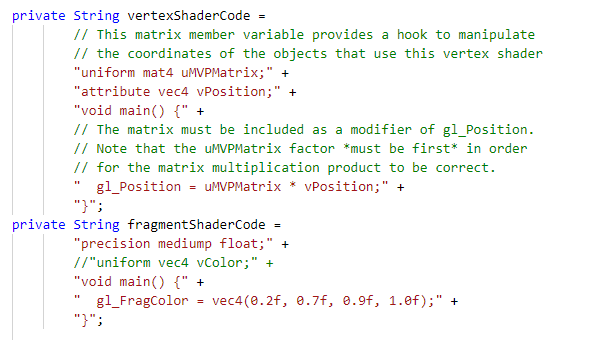
\includegraphics[width=5in]{figures/GLSL.png}
        \caption{Código en GLSL}
        \label{fig:codigoGLSL}
    \end{figure}
    \newpage    
    \item Otro aspecto a tener en cuenta es que OpenGL solo nos ofrece lo básico, no nos ofrece métodos para dibujar 
    directamente objetos, sino que hay que seguir un pipeline de procesos para conseguir dibujar algo (ver \autoref{fig:pipeline}).
    Esto consiste en pasar un array de números (cada tres para definir un punto) 
    a las tarjetas gráficas, establecer triángulos entre los puntos (más arrays de números) 
    definir colores a partir de los puntos (más arrays...), y con el código del shader, ejecutar 
    estos datos.
    \begin{figure}
        \centering
        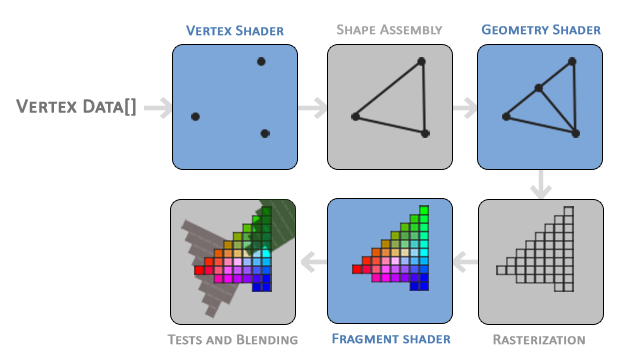
\includegraphics[width=4in]{figures/pipeline.png}
        \caption{Pipeline de la construcción de un modelo\cite{pipelineopengl}}
        \label{fig:pipeline}
    \end{figure}
    \item Por último, como sólo ofrece métodos básicos, no hay métodos de escritura de texto, y la forma que 
    encontramos para que funcione fue usar un bitmap con los caracteres (ver \autoref{fig:mapaBits}). Este fue el principal 
    motivo de rechazar esta tecnología ya que, dependiendo de la funcionalidad que se desee implementar, es necesario codificar a muy bajo nivel, lo que costaría mucho tiempo y esfuerzo.
    \begin{figure}
        \centering
        
\includegraphics[width=5in]{figures/bitmap-font.png}
        \caption{Mapa de bits de caracteres usado}
        \label{fig:mapaBits}
    \end{figure}
\end{enumerate}

\subsection{Vuforia + Unity} 
\label{makereference4.1.4}

    Para realizar este prototipo utilizamos Unity como herramienta básica para realizar la aplicación y Vuforia para dar soporte a la realidad aumentada.
    El prototipo a desarrollar consistió en un modelo 3D de un dragón que aparecía al detectar una imagen que previamente habíamos establecido como ``imagen objetivo''.

    \begin{figure}[H]
        \centering
        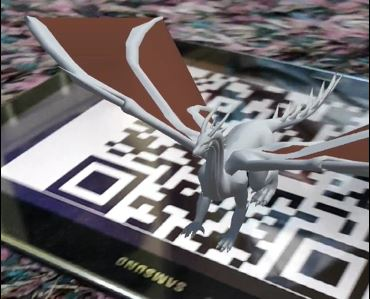
\includegraphics[width=5in]{figures/prototipoUnity.jpg}
        \caption{Modelo en 3D que aparecía al detectar la imagen}
    \end{figure}

Pese a que nadie del equipo había utilizado Unity previamente el resultado fue bastante positivo ya que:
\begin{enumerate}
    \item Unity resultó ser intuitivo y relativamente fácil en cuanto al aprendizaje de las funcionalidades básicas.
    \item Vuforia parecía estar muy probada e incluía de serie muchas funcionalidades.
    \item Vuforia tenía la opción de utilizar un Cloud para almacenar las imágenes objetivo.
\end{enumerate}


\subsection{Vuforia + Unity + Android} 
\label{makereference4.1.5}

Una vez realizado el prototipo en Vuforia con Unity comenzamos a investigar cómo realizar el resto de la aplicación que no requería de Realidad Aumentada.
Hasta este momento teníamos claro que Vuforia con Unity era la mejor combinación para realizar la parte de realidad aumentada. Sin embargo, tras realizar pruebas desarrollando en Unity interfaces y lógica nos dimos cuenta de que Unity no era igual de intuitivo ni eficaz a la hora de realizar estas tareas que necesitábamos para desarrollar el resto de la aplicación que no necesitaba Realidad Aumentada.
Por este motivo intentamos buscar la opción de realizar una aplicación en la que la realidad aumentada estuviese diseñada en Unity con Vuforia y el resto de la aplicación en Android (ver \autoref{fig:botonAndroidUnity}).

\begin{figure}[H]
    \centering
    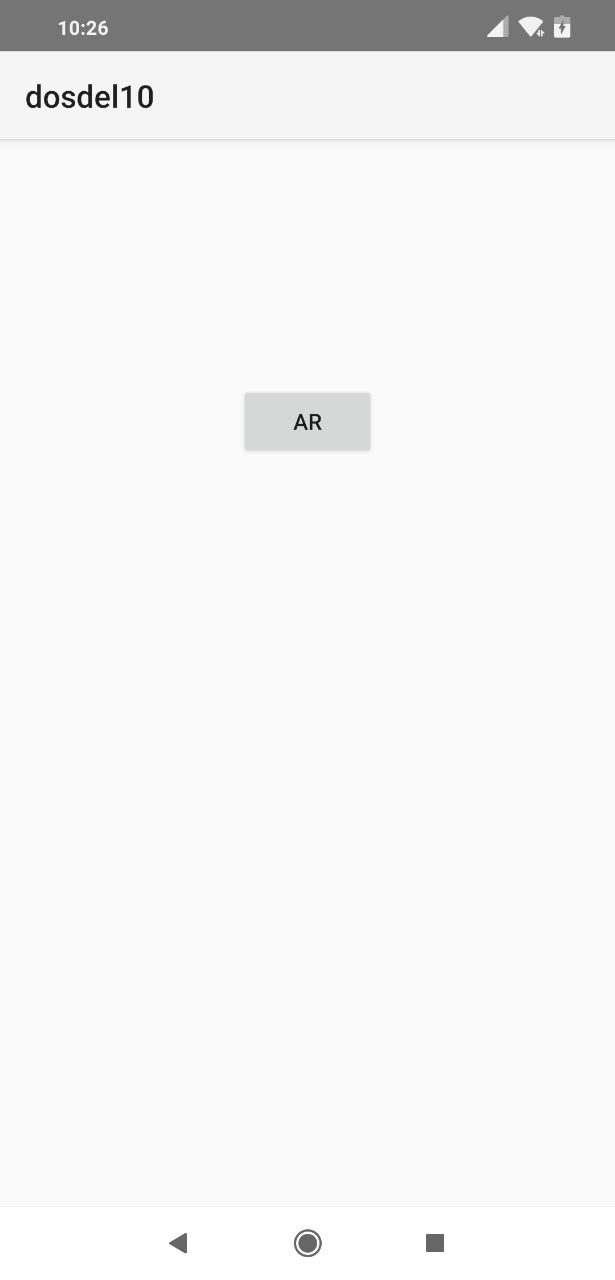
\includegraphics[height=4in]{figures/androidUnityVuforia.jpg}
    \caption{Botón que comunica Android con Unity}
    \label{fig:botonAndroidUnity}
\end{figure}

Finalmente conseguimos tener ambos proyectos independientes. La realidad aumentada se desarrollaba en Unity con Vuforia y se exportaba a un proyecto Android donde se encontraba el resto de la aplicación.
Esto nos permitía realizar la realidad aumentada con la herramienta que tras las primeras tomas de contacto habíamos comprobado que era la mejor (Unity con Vuforia) y del mismo modo realizar el resto de la aplicación con la mejor herramienta para esta parte (Android Studio).

Tras realizar este prototipo, consideramos que estas herramientas podrían ser las que usásemos en la aplicación final puesto que:
\begin{enumerate}
    \item Como ya habíamos descubierto en el prototipo anterior, Unity era una herramienta muy completa y junto con Vuforia nos proporcionaban todas las herramientas necesarias para cumplir con los casos de uso de Realidad Aumentada que teníamos en mente.
    \item Al haber encontrado la forma de combinar Unity y Android no teníamos que renunciar a ninguna de las dos herramientas. Lo que nos permitía explotar las cosas buenas de ambas herramientas.
    \item La comunicación entre Unity y Android era relativamente sencilla pese a ser dos proyectos distintos.
\end{enumerate}


\subsection{Server en Spring} 
\label{makereference4.1.6}

Para la realización de la parte backend de la aplicación explicada a continuación,
decidimos incorporar la tecnología de Spring para codificar un servicio web REST en Java
y el acceso a datos mediante MySQL. Para el prototipo seguimos un tutorial\cite{tutorialspring} de 3 partes para crear un servicio web REST
que gestionara una simple entidad de contactos de personas, con atributos como el nombre completo del contacto, su número de teléfono o su correo electrónico.

También se investigaron distintas formas de realizar el acceso a la base de datos desde el servidor, nos decantamos por una clase que nos ofrecía implementados los métodos básicos para crear, leer, actualizar y borrar datos. Además de la opción 
de poder crear nuestros propios métodos.

Para este prototipo decidimos usar MySQL como sistema de gestión de bases de datos relacional, aunque
a la hora de probar a levantar nuestro servidor de prueba tuvimos que rehacer este prototipo, además de adaptarlo para 
que gestionara entidades de películas, y que usara PostgreSQL.
\section{Arquitectura}
\label{makereference4.2}
En cuanto a la arquitectura usada en nuestra aplicación hemos adjuntado un esquema que podemos observar en la \autoref{fig:arquitectura}. Nuestra aplicación móvil estará implementada tanto en Android
como en Unity. La aplicación general está en Android, mientras que la parte de realidad aumentada está desarrollada en Unity y usa Vuforia. Para el reconocimiento
de imágenes con Vuforia usamos un almacenamiento en la nube gratuito.
Para la parte del servidor, hemos realizado una API Rest con Spring, usando además una base de datos relacional en PostgreSQL. La comunicación entre cliente y servidor se realiza mediante peticiones HTTP a 
nuestro servidor desplegado en Heroku el cual nos devolverá los datos en formato JSON y posteriormente los mapearemos a una clase Java.
\begin{figure}[H]
    \centering
    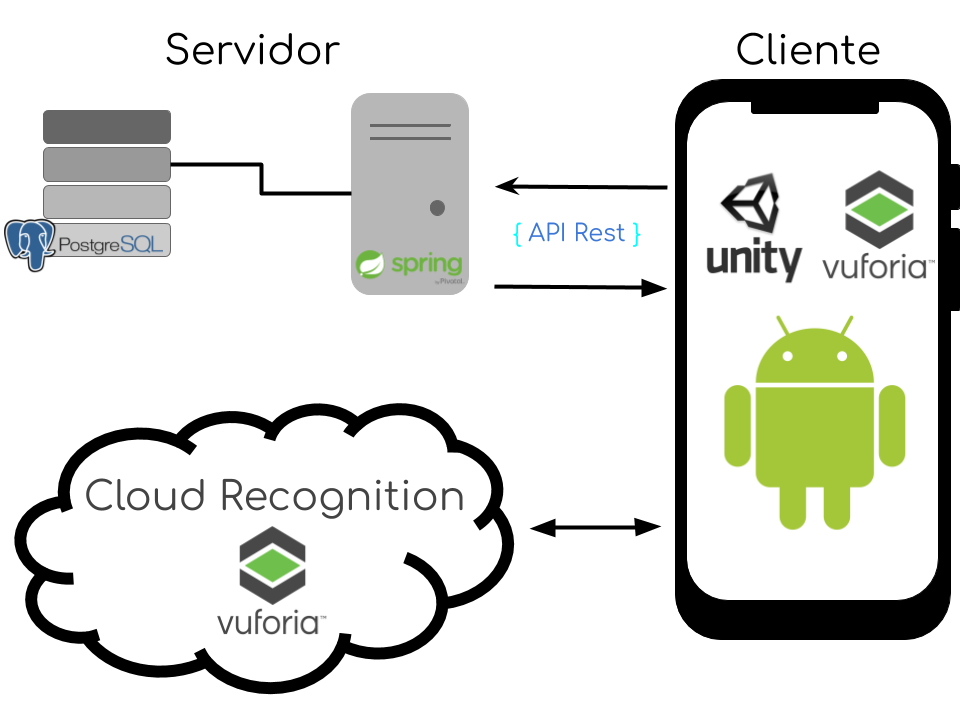
\includegraphics[width=6in]{figures/chapter-4/arquitectura.png}
    \caption{Arquitectura}
    \label{fig:arquitectura}
\end{figure}
\section{Servidor}
\label{makereference4.3}
Nuestro servidor está programado en Java, usando el framework Spring para la creación de una API Rest que, mediante peticiones HTTP y una base de datos relacional en PostgreSQL, nos proporcionará
toda la información necesaria para alimentar de datos a nuestro cliente. También se encuentra en el servidor la implementación del sistema de recomendación.
\subsection{Entidades}
\label{makereference4.3.1}
En el servidor tendremos todas las entidades que necesitamos
 (Ver \autoref{fig:modelo-ER}), estas son representadas
 mediante clases Java y anotaciones de JPA. Para facilitar el mapeo entre
 tablas de la base de datos y dichas entidades.
Hemos implementado las siguientes entidades:
\begin{figure}[H]
    \centering
    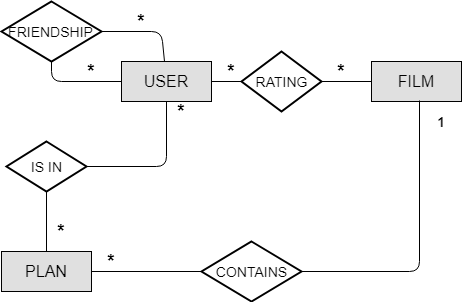
\includegraphics[width=6in]{figures/chapter-4/Entidades-ER.png}
    \caption{Modelo entidad-relación}
    \label{fig:modelo-ER}
\end{figure}
\begin{itemize}
    \item Film: entidad referente a las películas que guardamos, con su respectivo título, director, duración, valoración, url del tráiler, sinopsis, url de la imagen de la película, género, país y fecha de estreno.
    \item User: entidad para representar a los usuarios de la aplicación, con su nombre, foto, email y contraseña.
    \item Friendship: entidad para representar la relación de amistad entre usuarios.
    \item Plan: entidad para representar los planes. Estos poseerán una película, un usuario creador, fecha, hora, lugar, título, descripción y una lista de usuarios unidos.
    \item UserFilm: entidad intermedia para representar la relación de usuarios con películas, es decir, las películas que son guardadas por cierto usuario.
\end{itemize}
\subsection{Sistemas de recomendación}
\label{makereference4.3.2}
Implementamos el sistema de recomendación para obtener películas y planes
que pueden ser interesantes para cada usuario, en base a sus gustos.
Estas recomendaciones se utilizan en la parte de cliente y se muestran al
usuario a través de la interfaz.
La aplicación de Android se comunica con el servidor usando la
 API REST (Ver \autoref{makereference4.3.3}).
En la que disponemos de todas las búsquedas necesarias.
Los datos de las recomendaciones se guardan en una tabla de la base de datos.
Cada periodo de tiempo establecido previamente un procedimiento se ejecuta
 y actualiza la tabla para aplicar los nuevos datos guardados a las recomendaciones.
Este procedimiento usa una funcionalidad de la librería Mahout,
 para extraer los datos de valoraciones de usuarios a películas.
Con estos datos y usando una técnica de filtrado colaborativo genera las recomendaciones.
Como generar las recomendaciones es un proceso costoso y lento guardamos los
 resultados para ser utilizados.

\subsection{Controladores}
\label{makereference4.3.3}
Para cada una de estas entidades necesitamos una clase Controller, que actuará de controlador para saber redirigir cada petición HTTP a su correspondiente servicio de aplicación, donde se aplicará la lógica del negocio, comprobando 
que los datos son correctos y obteniendo, modificando o creando elementos en la base de datos a través de las clases Repository correspondiente a cada entidad.
A la búsqueda por ID tuvimos que añadir la búsqueda por UUID en usuarios y películas.
El ID es necesario para utilizarlo en el sistema de recomendación de Mahout y
el UUID es necesario para el reconocimiento de imágenes de Vuforia.
Las distintas peticiones HTTP que realizamos son las siguientes:

\begin{center}
    \begin{tabularx}{1\textwidth}{@{\extracolsep{\fill}} | l | l | X |} \hline
    \multicolumn{3}{|c|}{Film} \\ \hline
    Obtener todas las películas & GET & /films/ \\ \hline
    Guardar una película & POST & /films/ \\ \hline
    Actualizar una película & PUT & /films/ \\ \hline
    Buscar una película por su nombre & GET & /films/search/\{name\} \\ \hline
    Buscar una película por su id & GET & /films/\{id\} \\ \hline
    Buscar una película por su uuid & GET & /films/uuid/\{uuid\} \\ \hline
    Borrar una película & DELETE & /films/\{id\} \\ \hline
    \end{tabularx}
\end{center}

\begin{center}
    \begin{tabularx}{1\textwidth}{@{\extracolsep{\fill}} | l | l | X |} \hline
    \multicolumn{3}{|c|}{User} \\ \hline
    Obtener todos los usuarios & GET & /users/ \\ \hline
    Guardar un usuario & POST & /users/ \\ \hline
    Actualizar un usuario & PUT & /users/ \\ \hline
    Buscar un usuario por su nombre & GET & /users/search/\{name\} \\ \hline
    Buscar un usuario por su id & GET & /users/\{id\} \\ \hline
    Buscar un usuario por su uuid & GET & /users/uuid/\{uuid\} \\ \hline
    Borrar un usuario & DELETE & /users/\{id\} \\ \hline
    Obtener amistades de un usuario & GET & /users/\{id\}/friendships \\ \hline
    Obtener amigos de un usuario & GET & /users/\{id\}/friends \\ \hline
    Obtener planes de un usuario & GET & /users/\{id\}/plans \\ \hline
    Obtener películas que gustan a un usuario & GET & /users/\{id\}/films \\ \hline
    Login de un usuario & POST & /users/login \\ \hline
    \end{tabularx}
\end{center}

\begin{center}
    \begin{tabularx}{1\textwidth}{@{\extracolsep{\fill}} | l | l | X |} \hline
    \multicolumn{3}{|c|}{UserFilm} \\ \hline
    Obtener todas las valoraciones & GET & /user-films/ \\ \hline
    Guardar valoración & POST & /user-films/ \\ \hline
    Actualizar valoración & PUT & /user-films/\{userId\}/\{filmId\}/rate/\{rating\} \\ \hline
    Buscar una valoración & GET & /user-films/\{userId\}/\{filmId\} \\ \hline
    Borrar una valoración & GET & /user-films/\{id\} \\ \hline
    \end{tabularx}
\end{center}
\begin{center}
    \begin{tabularx}{1\textwidth}{@{\extracolsep{\fill}} | l | l | X |} \hline
    \multicolumn{3}{|c|}{Recommender} \\ \hline
    Obtener todas las recomendaciones & GET & /recommendations/ \\ \hline
    Obtener películas random & GET & /recommendations/random \\ \hline
    Obtener películas más relevantes & GET & /recommendations/trending \\ \hline
    Obtener películas más nuevas & GET & /recommendations/premiere \\ \hline
    Recomendaciones para un usuario & GET & /recommendations/\{id\} \\ \hline
    Obtener las recomendaciones de planes & GET & /recommendations/\{id\}/plans/\{friend\} \\ \hline
    Borrar todas las recomendaciones & DELETE & /recommendations/ \\ \hline
    Borrar todas las recomendaciones & DELETE & /recommendations/\{id\} \\ \hline
    \end{tabularx}
\end{center}
\begin{center}
    \begin{tabularx}{1\textwidth}{@{\extracolsep{\fill}} | l | l | X |} \hline
    \multicolumn{3}{|c|}{Images} \\ \hline
    Obtener imagen & GET & /\{image\}/ \\ \hline
    \end{tabularx}
\end{center}
\begin{center}
    \begin{tabularx}{1\textwidth}{@{\extracolsep{\fill}} | l | l | X |} \hline
    \multicolumn{3}{|c|}{Friendships} \\ \hline
    Obtener todas las amistades & GET & /friendships/ \\ \hline
    Petición de amistad & POST & /friendships/\{requesterId\}/\{friendId\}/request \\ \hline
    Aceptación de amistad & POST & /friendships/\{requesterId\}/\{friendId\}/accept \\ \hline
    Declinar amistad & DELETE & /friendships/\{requesterId\}/\{friendId\}/decline \\ \hline
    Eliminar amistad & DELETE & /friendships/\{requesterId\}/\{friendId\} \\ \hline
    \end{tabularx}
\end{center}
\begin{center}
    \begin{tabularx}{1\textwidth}{@{\extracolsep{\fill}} | l | l | X |} \hline
    \multicolumn{3}{|c|}{Plans} \\ \hline
    Obtener todos los planes & GET & /plans/ \\ \hline
    Guardar un plan & POST & /plans/ \\ \hline
    Unirse a un plan & PUT & /plans/\{id\}/join/\{userId\} \\ \hline
    Eliminar un plan & DELETE & /plans/\{id\} \\ \hline
    Obtener planes por id & GET & /plans/\{id\} \\ \hline
    Obtener los usuarios unidos a plan & GET & /plans/\{id\}/joined-users \\ \hline
    Obtener los usuarios de un plan & GET & /plans/\{id\}/users \\ \hline
    Buscar un plan por nombre & GET & /plans/search/\{title\} \\ \hline
    \end{tabularx}
\end{center}

\section{Cliente}
\label{makereference4.4}
Nuestra aplicación está implementada principalmente en Android, las interfaces principales para el uso de los planes, recomendaciones y acceso a la información de las películas guardadas han sido desarrolladas mediante Android Studio. Sin embargo,
la parte del cliente que otorga el gran valor a nuestra aplicación está desarrollada en Unity y el uso de Vuforia, todas las escenas que aparecen al reconocer carteles de películas e imágenes de usuarios fueron implementadas de esta forma.
La parte de la aplicación realizada en Unity, utiliza una serie de clases de la parte desarrollada en Android para realizar las peticiones al servidor y así poder mostrar información específica cuando se reconoce una cierta imagen.
Al principio la parte de Android implementaba la obtención de datos del servidor que necesitaba y la parte de Unity la suya. Después decidimos implementar la obtención de datos únicamente en Android y hacer usarlo desde Unity para tener mejor control y no duplicar soluciones al mismo problema.
Las imágenes que mostramos en la parte de Android se almacenan en el mismo servidor.


Como la mayor parte de la aplicación está implementada en Android Studio, la estructura de ésta se adapta a lo que ofrece el IDE, consistiendo en el flujo de unas actividades y fragmentos que explicaremos a continuación.


\subsection{Actividades}
\label{makereference4.4.1}
Son los componentes de la aplicación que representan una pantalla con la que
 los usuarios pueden interactuar para realizar una determinada
 acción (ver \autoref{fig:activity}).
\begin{figure}[H]
    \centering
    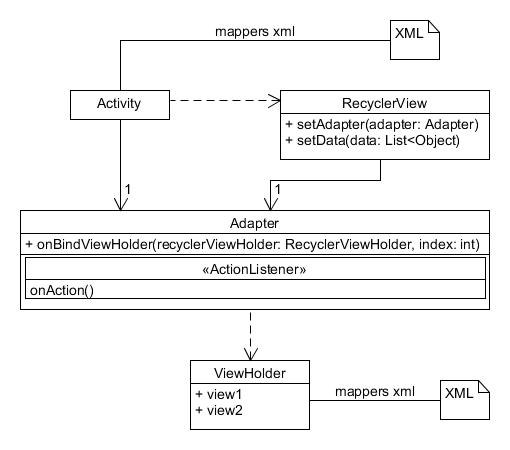
\includegraphics[width=6in]{figures/chapter-4/Activity.jpeg}
    \caption{Actividades}
    \label{fig:activity}
\end{figure}

Entre nuestras actividades podemos destacar dos: 
\begin{itemize}
    \item MainActivity: La primera actividad (actividad principal) que se activa al iniciar la aplicación, la cual comprueba el estado de sesión del usuario, si está logueado se queda en la actividad, y si no, se redirige al usuario a otra actividad llamada LoginActivity que mediante un formulario muy simple nos permite iniciar sesión o registrarnos. En MainActivity se encuentra un paginador (ViewPager) de 3 fragmentos, donde cada fragmento representa las interfaces de planes, recomendaciones y películas guardadas correspondientemente. Podemos observarlo en la \autoref{fig:listaPlanes}, \autoref{fig:lista_peliculas} y \autoref{fig:recomendaciones_1} del \autoref{makereference3}.
    \item UnityPlayerActivity: Se trata de una actividad especial que nos permite comunicar la parte desarrollada en Unity con nuestro proyecto Android. Aquí se encuentran llamadas a funciones desde la parte de Unity, se realizan las órdenes y se devuelven a Unity.
\end{itemize} 

\subsection{Adaptadores}
\label{makereference4.4.2} 
Son elementos de manipulación de datos que se aplican a vistas y componentes. En el proyecto se les ha dado mucho uso a las vistas de tipo RecyclerView para representar listas de objetos. Para manejar los datos de cada elemento de la lista, se ha utilizado un RecyclerView.Adapter, el cual manipula cada dato correspondiente a un elemento de la lista. También se han creado otros adaptadores, como uno para manejar tres fragmentos dentro de una actividad, como hemos dicho anteriormente al describir la actividad principal (MainActivity).

\subsection{Comandos}
\label{makereference4.4.3}
Aquí se encuentran todos los elementos relacionados con el patrón comando (ver \autoref{fig:comando}).
Ha sido diseñado para realizar la conexión con la parte del proyecto desarrollado en Unity.
Al principio las peticiones al servidor se realizaban tanto en Android como en
Unity. Esto causaba que tuviéramos implementaciones duplicadas y originaba
 problemas si había que modificar estos métodos, porque era necesario aplicar los
 cambios en ambas capas.
Decidimos utilizar desde Unity los métodos de Android para resolver el problema.
Para evitar que Unity tuviera múltiples dependencias con la capa de Android,
 decidimos aplicar el patrón comando.
Este patrón nos permite abstraer la capa de Android con la capa de Unity y
 minimizar las dependencias que eran necesarias.

\begin{figure}[H]
    \centering
    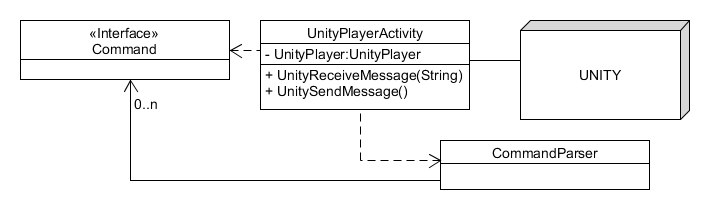
\includegraphics[width=6in]{figures/chapter-4/Command.jpeg}
    \caption{Patrón comando}
    \label{fig:comando}
\end{figure}



\subsection{Entidades}
\label{makereference4.4.4}
Todos los modelos de datos que podemos recibir del servidor, los cuales hemos descrito anteriormente en este capítulo, en la Sección 4.3, son representados por entidades en nuestro proyecto de Android, con los mismos atributos que tienen sus entidades correspondientes en el servidor.

\subsection{Fragmentos}
\label{makereference4.4.5}
Representan un comportamiento o una parte de la interfaz de usuario en una actividad.
Se utilizan para formar una vista compuesta de paginación en una actividad. 
Aquí es donde tendremos los 3 componentes principales de nuestra aplicación, la actividad referente a mis planes, la actividad de las recomendaciones y la de mis películas.

\subsection{Petición de servicios}
\label{makereference4.4.6}
Se trata de un conjunto de clases que solo poseen métodos estáticos para llevar
 a cabo peticiones HTTP al servidor. Se ha creado una clase genérica para la
 creación y llamada de peticiones HTTP, se ha diseñado de manera que las
 respuestas se devuelvan en forma de callback para un uso más sencillo
 (ver \autoref{fig:server}).
\begin{figure}[H]
    \centering
    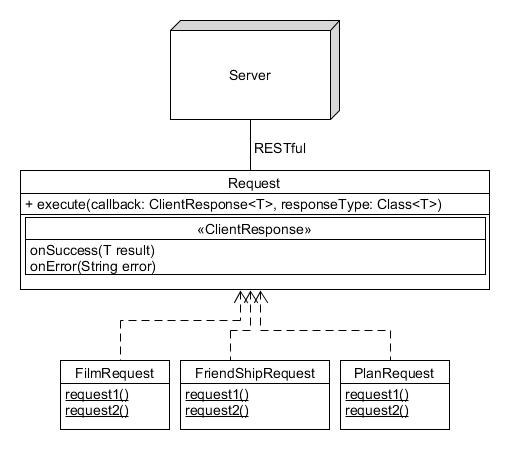
\includegraphics[width=6in]{figures/chapter-4/Request.jpeg}
    \caption{Petición de servicios}
    \label{fig:server}
\end{figure}
Los servicios que hemos implementado son los siguientes:
\begin{itemize}
    \item FilmRequest: servicio encargado de realizar las peticiones sobre películas al servidor, como podría ser buscar una película por su ID.
    \item FriendshipRequest: servicio responsable de obtener los datos relacionados a las relaciones entre amistad, como podría ser aceptar una petición o comprobar si dos usuarios son amigos.
    \item PlanRequest: servicio cuya finalidad es la de conseguir la información relacionada con los planes, como podría ser la operación de crear un plan y unirse o salirse de uno ya existente.
    \item RecommendationRequest: este servicio se ocupa de obtener las distintas recomendaciones de películas y planes de un usuario.
    \item UserFilmRequest: servicio creado para obtener la información referente a ciertos métodos de la relación entre películas y usuarios. Por ejemplo, con este servicio podríamos guardar una película como favorita de un usuario. También es usado para cuando un usuario valora cierta película.
    \item UserRequest: servicio que nos permite obtener todo lo relacionado con los usuarios, ya sean sus perfiles, los amigos de un usuario, los planes en los que está o las películas que ha guardado.
\end{itemize}

\subsection{Vistas}
\label{makereference4.4.7}
Entre los componentes que ofrece Android existen algunas funcionalidades no soportadas. Por ello hemos creado componentes personalizados para satisfacer estas funcionalidades:
\begin{itemize}
    \item AnchorVisibilityBehavior: Implementa el comportamiento de los elementos que aparecen y desaparecen en las actividades, por ejemplo, en la \autoref{fig:info_planes} tenemos un botón para la información de la película pero al hacer el scroll hacia abajo, en la \autoref{fig:info_planes_1}, vemos que éste desaparece.
    \item CustomViewPager: el ViewPager es lo que usamos en la MainActivity para colocar los tres fragmentos. Se crea esta clase para desactivar la acción de cambiar entre fragmentos al deslizar con el dedo en la pantalla del smartphone. Esto nos daba problemas debido a que en el fragmento de las recomendaciones tenemos elementos con scroll horizontal y la acción de deslizar con el dedo en la pantalla interfería.
    \item ExpandableTextView: Es una clase que extiende de un TextView, se le añade un método para que cuando haya mucho texto, se pueda acortar. Además dispone de un botón para expandir.
\end{itemize} 

\section{Despliegue}
\label{makereference4.6}
El servidor puede desplegarse como un Docker o en Heroku.
Para el desarrollo del proyecto hemos utilizado Heroku por la facilidad y
comodidad que ofrece. 
Usamos una cuenta gratuita que nos permite un alojamiento limitado con las
 características suficientes para el desarrollo del proyecto.
Utilizamos un despliegue automático que al realizar cambios en una rama del
 repositorio de GitHub, Heroku descarga esos cambios y lo despliega en el servidor.
En la \autoref{app:heroku} encontramos una guía de como desplegar la
aplicación con tu usuario de Heroku. En la \autoref{app:docker} vemos como
desplegar la aplicación en un Docker.

\section{Herramientas de trabajo}
\label{makereference4.7}
Las distintas herramientas de trabajo que hemos decidido usar para que el trabajo realizado fuera más eficiente son las siguientes:
\begin{itemize}
    \item Telegram: hemos usado esta aplicación de mensajería para poder comunicarnos entre todos los miembros pertenecientes al proyecto, ya fuera para la sugerencia de ideas o que un bot de GitHub nos avisara de los cambios en los distintos repositorios que hemos creado. 
    \item Slack: esta otra herramienta de comunicación nos ha permitido crear canales específicos para cada parte de nuestro proyecto y así poder clasificar las conversaciones que teníamos por temas, por ejemplo, tenemos un canal para hablar solo de la parte backend, otro para hablar de la parte de realidad aumentada, etc. Cosa que Telegram no nos permitía y resultaba lioso encontrar ciertos temas o puntos de nuestras conversaciones. 
    \item Trello: nos ha servido como apoyo para realizar nuestros sprints, Trello nos ofrece la posibilidad de crear un tablero para escribir tareas a modo de post-it y asignarlas a usuarios que estén dentro del tablero, así sabemos qué tipo de tareas ha realizado o está realizando cada miembro en todo momento.
    \item GitHub: todos nuestros repositorios están en GitHub, lo que nos permite subir cambios y trabajar en paralelo en distintas ramas, agilizando así nuestro trabajo y otorgándonos un control de versiones muy estable.
    \item Visual Studio Code: utilizamos este editor de código junto con la extensión de LaTeX Workshop para escribir la memoria en LaTeX.
    \item Android Studio: usamos este IDE para construir la aplicación Android que además nos dota de herramientas de depuración.
    \item Google Drive: almacenamiento en la nube donde tenemos toda la información relevante para el TFG.
    \item Heroku: plataforma en la que desplegamos nuestra aplicación de servidor.
    \item Unity: Utilizamos esta plataforma de desarrollo para construir la parte de la aplicación relacionada con Realidad Aumentada.
    \item Visual Studio: Utilizamos Visual Studio para codificar los scripts en C\# necesarios para el funcionamiento de la parte de realidad aumentada en Unity.
    \item Postman: aplicación para el envío de peticiones HTTP REST, que utilizamos para depurar los servicios de Spring.
    \item MockFlow: herramienta online para el diseño de mockups, nosotros la utilizamos para el diseño de las vistas de la aplicación Android.
\end{itemize}

\section{Conclusiones}
\label{makereference4.8}
A continuación, mostraremos una lista de todas las dificultades encontradas a la hora de implementar nuestra aplicación:
\begin{itemize}
    \item Diseño de las interfaces para que fueran familiares e intuitivas para el usuario. Tuvimos que rehacer muchas veces los distintos bocetos de las interfaces ya que no eran intuitivos para los usuarios. Gracias a las sugerencias que se nos iban haciendo conseguimos mejorarlas bastante.
    \item Desconocimiento del entorno de desarrollo y peculiaridades del desarrollo de aplicaciones en Android. Para resolver nuestro desconocimiento de Android realizamos una serie de prototipos y buscamos tutoriales que nos sirvieran como ejemplo para desarrollar cada parte de nuestra aplicación.
    \item Incompatibilidad de realización de peticiones HTTP en ciertas versiones de Android. Tras probar la aplicación en un smartphone con versión de Android 9.0 descubrimos que los permisos para hacer peticiones de este tipo a un servidor no funcionaban con la configuración inicial de nuestro proyecto. Para solucionarlo cambiamos una serie de líneas de código en nuestro archivo AndroidManifest.xml para solventarlo.
    \item Problemas a la hora de intentar desplegar el servidor de forma correcta para que fuera accesible siempre. Para que el servidor estuviera siempre levantado se nos ocurrió realizar su despliegue en Heroku para así poder realizar peticiones en cualquier momento desde la app.
    \item Poca familiaridad con el uso de Unity y el lenguaje C\# para realizar la parte de realidad aumentada. Para familiarizarnos con el entorno implementamos una serie de prototipos y buscamos tutoriales que nos sirvieran como guía para diseñar nuestra parte de realidad aumentada. 
    \item Caducidad de las licencias gratuitas para el uso del Cloud de Vuforia. La solución a este problema fue muy simple, crearnos cuentas nuevas cada vez que se acabara la licencia para poder seguir accediendo a este servicio.
    \item Primera vez usando el framework de Spring para la realización de una API Rest. Su solución fue seguir un tutorial paso a paso para crearlo con una sola entidad e ir ampliándolo a todas las entidades que necesitaba nuestra aplicación.
    \item Comunicación entre la parte cliente en Android y el servidor. Conseguimos realizar servicios en Android que realizaban las peticiones al servidor de forma asíncrona, obteniendo su resultado en una función callback para usar dicha información como correspondiera en cada caso.
    \item Comunicación entre la parte cliente en Unity con la parte cliente en Android. Para abstraer la lógica desarrollada en Android a la de Unity implementamos clases que usaban el patrón Command para facilitar la comunicación entre estas dos partes de nuestro proyecto.
    \item Rendimiento en cuanto al reconocimiento de ciertas imágenes, sobre todo de personas, debido a la calidad de las mismas. El Cloud de Vuforia no las reconoce tan fácilmente como las de carteles de películas. Para arreglarlo tuvimos que buscar imágenes de usuarios con una mejor calidad para facilitar a la librería su reconocimiento, finalmente optamos por poner imágenes de los integrantes del proyecto durante el desarrollo de la aplicación.
    \item Almacenamiento de imágenes en Google Drive y su obtención desde Android y Unity, junto con el retardo que esto produce. Para no tener las imágenes de los usuarios en la aplicación se nos ocurrió guardarlas en Google Drive y obtenerlas con la librería de Picasso de Android, pero esto era muy lento y decidimos guardarlas en el mismo servidor.
    \item Incompatibilidades con las nuevas actualizaciones de Unity. Hemos tenido cuidado con no actualizar el IDE de Unity porque nuestro proyecto quedaría obsoleto, ya nos vimos en la situación de que uno de los miembros tenía una versión superior a la de los demás y tuvimos que rehacer lo que habíamos implementado.
\end{itemize}